\documentclass[11pt]{article}
\usepackage[breaklinks=true]{hyperref}
\usepackage{color}
\usepackage{amsmath,amssymb,amsthm}
\usepackage{natbib}
\usepackage{array}
\usepackage{booktabs, multicol, multirow}
\usepackage[nohead, margin=1in]{geometry}
\usepackage[singlespacing]{setspace}
\usepackage{graphicx}


\newtheorem{theorem}{Theorem}[section]
\newtheorem{lemma}[theorem]{Lemma}
\newtheorem{assumption}{Assumption}

\newcommand{\beq}{\begin{equation}}
\newcommand{\eeq}{\end{equation}}
\newcommand{\bit}{\begin{itemize}}
\newcommand{\eit}{\end{itemize}}

\newcommand{\todo}[1]{{\color{red}{TO DO: \sc #1}}}

\newcommand{\reals}{\mathbb{R}}
\newcommand{\integers}{\mathbb{Z}}
\newcommand{\naturals}{\mathbb{N}}
\newcommand{\rationals}{\mathbb{Q}}

\newcommand{\ind}{\mathbb{I}} % Indicator function
\newcommand{\pr}{\mathbb{P}} % Generic probability
\newcommand{\ex}{\mathbb{E}} % Generic expectation
\newcommand{\var}{\textrm{Var}}
\newcommand{\cov}{\textrm{Cov}}

\newcommand{\normal}{N} % for normal distribution (can probably skip this)
\newcommand{\eps}{\varepsilon}
\newcommand\independent{\protect\mathpalette{\protect\independenT}{\perp}}
\def\independenT#1#2{\mathrel{\rlap{$#1#2$}\mkern2mu{#1#2}}}
\newcommand{\argmax}{\textrm{argmax}}
\newcommand{\argmin}{\textrm{argmin}}
\renewcommand{\baselinestretch}{1.5}

\title{A Comparison of Parametric and Permutation Tests for Regression Analysis of Randomized Control Trials}
\author{Kellie Ottoboni \\
Department of Statistics; Berkeley Institute for Data Science\\
University of California, Berkeley\\ [.2in]
Luigi Salmaso\\
Department of Management and Engineering \\
University of Padova \\ [.2in]
Fraser Lewis \\
RB
}\date{Draft \today}
\begin{document}
\maketitle

\newpage

\begin{abstract}
\noindent\textbf{Background:}
In clinical trials, the standard method of measuring the effectiveness of one treatment over another is a parametric analysis of covariance (ANCOVA), a special case of linear regression which incorporates stratification.
The method relies on strong, untestable assumptions about the data-generating process such as constant treatment effects across groups, normality of errors, and homoskedasticity.
The effectiveness of the treatment is decided by the p-value from this hypothesis test, which may not be valid if the assumptions for ANCOVA are not met.
We would like to understand which assumptions may be relaxed or violated for the ANCOVA to remain valid (but potentially less powerful).

\noindent\textbf{Methods:}
Permutation tests present such an opportunity: they require only minimal assumptions which are often guaranteed by the randomization that was conducted.
In contrast to parametric tests, which rely up on strong assumptions to obtain a null distribution with a simple closed form, with permutation tests one uses the assumption of exchangeability or randomization to construct approximate null distributions by simulation.
These tests are exact, even in finite samples.
We compare ANCOVA to several permutation tests based on linear models, all of which control for pretreatment covariates to increase power and precision.

\noindent\textbf{Results:}
Our simulations show that the permutation methods maintain power comparable to the ANCOVA in randomized trials.
We illustrate the use of permutation tests alongside the parametric ANCOVA using data from a clinical trial conducted across eight sites,
each having a different numbers of patients.

\noindent\textbf{Conclusions:}
These results suggest that the parametric ANCOVA and linear model permutation tests perform similarly, even when not all assumptions for the parametric test are met.


\end{abstract}

% keywords: permutation test, linear model, ANOVA
\newpage

\section{Background}
A hypothesis test is a statistical method for determining whether observed data is consistent with a belief about the process that generated the data.
Medical experiments use hypothesis testing to assess the evidence that a treatment has an effect on one or more clinically relevant outcomes.
The simplest version of this experiment, which involves randomly assigning two treatments to a fixed number of individuals in a group and measuring a single outcome, has been studied for nearly a century (see \citet{fisher_design_1935} and \citet{neyman_application_1923} for early references).
One can conduct hypothesis tests and construct confidence intervals for the estimated treatment effect
by exploiting the fact that the difference in average outcomes between the two treatment groups is asymptotically normal with a variance that can be estimated from the data.

Randomized experiments in the real world are rarely this simple:
individuals are heterogeneous with respect to pretreatment covariates,
there may be more than two treatments under study,
they may not take the treatment they are assigned or may drop out of the study,
and an individual's assignment to treatment may affect others' outcomes.
Techniques have been developed to deal with each of these issues.
In this paper, we focus on the first.

Random assignment of treatment ensures that pretreatment covariates are balanced between treatment groups on average, across all possible randomizations.
However, in any particular randomization, there may be imbalances.
If the imbalanced covariates are associated with the outcome, then even when there is no effect of treatment, we may observe differences in outcomes between treatment groups.
Controlling for such baseline covariates can reduce the variability of estimated treatment effects and yield more powerful hypothesis tests. \todo{cite}

Stratification is one method for controlling for covariates that are known a priori to be associated with the outcome.
Individuals are divided into groups based on levels of this covariate, and random assignment of treatments is conducted within each group, independently across groups.
This guarantees that the stratification variable is balanced between treatment groups.
The stratification is done \textit{before any outcome data is collected}.
A common stratification variable in clinical experiments is location:
individuals often come from many sites because it is difficult to recruit a sufficient number of participants at one doctor's office or hospital.
As with other pretreatment covariates, outcomes may vary across strata due to factors unrelated to individuals.
Controlling for stratum can have the same beneficial effects as controlling for other pretreatment covariates.

Linear regression is another common way to control for baseline covariates.
It is done \textit{after} data are collected and outcomes are observed.
Whereas stratification guarantees balance on the stratifying variable, other covariates may be imbalanced, so stronger modeling assumptions are needed to balance them after the fact.
The idea of linear regression is to project the outcomes onto a plane which describes each variable's relationship to the outcome.
The coefficient of any particular variable answers the question, if we were to hold fixed all other covariates and increase this variable by one unit, how much would we expect the outcome to change?
This model posits a linear relationship between covariates, treatment, and outcome; 
if the true relationship is not linear, then regression only estimates the best linear approximation to the conditional expectation of the outcome.
When controlling for strata, such as location, it is standard to use analysis of covariance (ANCOVA), a particular case of linear regression which allows each stratum to have its own mean outcome level.
This amounts to choosing the plane of best fit for the data, allowing each stratum to have a different intercept but enforcing that the slope is the same for each.

Hypothesis testing of estimated coefficients requires even stronger assumptions than linearity, such as Gaussian, homoskedastic errors.
When this holds, a regression coefficient scaled by its estimated variance follows Student's $t$ distribution.
Thus, if we believe the linear model is correctly specified, a hypothesis test for a treatment effect amounts to a hypothesis test of the coefficient for treatment in the ANCOVA, and can be evaluated analytically and quickly.
However, the assumptions necessary for the coefficient to be $t$ distributed are clearly violated in many cases:
when the data are discrete or ordinal, when the treatment has a differential effect across strata, and when measurement error sizes differ across strata.
Furthermore, the hypothesis test implicitly assumes that the data were sampled at random from some underlying population, when in fact,
medical experimenters rarely recruit patients this way.

Permutation testing is an alternate approach (\cite{fisher_design_1935, pitman_significance_1937,pitman_significance_1938}).
Deliberate randomization induces a distribution for any test statistic under the null hypothesis that treatment has no effect on the outcome:
the randomization scheme provides information about all possible ways that treatment may have been assigned 
and the null hypothesis tells us what each individual's response would be regardless of the assignment (namely, it would be the same).
One determines how ``extreme'' the observed test statistic is relative to this randomization distribution, rather than a parametric reference distribution, such as Student's $t$ or the Gaussian.
Such a test is exact, meaning that it controls the type I error rate at the pre-specified level, even in finite samples, whereas parametric hypothesis tests based on asymptotic approximations do not always guarantee good finite sample properties.
Permutation tests achieve this by operating conditional on the observed sample; the resulting inference applies to the sample at hand, but does not necessarily generalize to other groups of individuals.
In the past, parametric tests were necessary because asymptotic approximations were the only computationally feasible way to estimate distributions. 
Now, computational power is no longer a barrier to finding exact (or exact to pre-specified precision) randomization distributions.
In most cases, a randomization test is preferable to a parametric one:
``[a] corresponding parametric test is valid only to the extent that it results in the same statistical decision [as the randomization test]'' (\cite{bradley_distribution_1968}).

There is no hard and fast rule describing the rate at which parametric tests approach the exact permutation solution, as they are both highly dependent on the particular data observed.
On the one hand, some argue that violations of parametric test assumptions necessitate the use of permutation methods.
\citet{ludbrook_why_1998} point out that medical trials rarely follow the population sampling model implicit in parametric methods.
However, the parametric and nonparametric tests seem to perform similarly in most simulations, even when data violate the assumptions of the parametric method.
Medical trials studying pain or perceived severity scores often use Likert scale data, which is discrete and does not match the normality assumptions of parametric tests.
However, \citet{winter_five-point_2010} found that the two sample $t$ test and Mann-Whitney test had comparable Type I and II error rates for five-point Likert scale data, suggesting that the violation of normality does not entirely invalidate the parametric test.
\todo{what other linear model comparisons have people done?}
Most similar to our question of study, \citet{vickers_parametric_2005} compared the parametric ANCOVA to the Mann-Whitney rank test in the context of randomized experiments, finding that except in extreme situations, ANCOVA outperformed the nonparametric test.


In this paper, we review hypothesis tests for a treatment effect which incorporate covariate adjustment to increase power.  
We focus on ANCOVA and its permutation counterparts, comparing their performance in different scenarios, and illustrating their application with a clinical dataset.
We find in simulations that even when assumptions are not satisfied, the parametric and permutation tests have comparable power to detect a treatment effect.
We apply each of the methods to data from a clinical trial seeking to compare the performance of two treatments for gastroesophageal reflux disease (GERD).
We conclude by discussing implications of these results for practitioners.

\section{Methods}
% The methods section should include:

%the aim, design and setting of the study
%the characteristics of participants or description of materials
%a clear description of all processes, interventions and comparisons. Generic drug names should generally be used. When proprietary brands are used in research, include the brand names in parentheses
%the type of statistical analysis used, including a power calculation if appropriate

\subsection{Problem and notation \todo{what do others call this?}}
Suppose we randomly assign two treatments labelled $0$ and $1$ to a group of individuals.
We are interested in comparing the relative effectiveness of treatment 1 to treatment 0.
Let $Z$ indicate treatment assignment, 0 or 1, 
$Y$ denote the observed outcome of interest,
and $X$ be a pretreatment covariate that is observed and associated with the outcome.
For expository clarity, we suppose that $X$ is univariate, but all results are easily extended to the case when $X$ is multivariate.
Suppose there is a categorical pretreatment variable with $J$ levels used to stratify individuals. 

We observe $\{Y_{ij}, Z_{ij}, X_{ij}\}$ for individuals $i = 1, \dots, n_j$, in strata $j = 1, \dots, J$.
All individuals have two potential outcomes, $Y_{ij}(1)$ and $Y_{ij}(0)$, representing their responses to treatments $1$ and $0$, respectively.
We can never observe both; random assignment of treatment reveals $Y_{ij} = Z_{ij}Y_{ij}(1) + (1-Z_{ij})Y_{ij}(0)$.

We are interested in the differences in potential outcomes $Y_{ij}(1) - Y_{ij}(0)$.
This difference represents the effect of treatment for individual $i$ in group $j$: it is the difference between what we would have observed under treatment 1 and what we would have observed under treatment $0$.\footnote{
Depending on the method of analysis one chooses, various functions of these differences will be considered.
Any of these quantities may be of clinical interest; it is a matter of philosophy which one prefers.}
A typical problem is to estimate the average of differences $Y_{ij}(1) - Y_{ij}(0)$.
Instead of estimation, we will focus on hypothesis testing for whether these differences are nonzero.

\subsection{Parametric ANCOVA}

The model is

\begin{equation}\label{eqn:ancova}
Y_{ij} = \alpha_j + \beta X_{ij} + \gamma Z_{ij} + \eps_{ij}
\end{equation}

\noindent where $\alpha_j$ is a fixed effect for stratum $j$, $\beta$ is the coefficient for the pretreatment covariate,
$\gamma$ is the coefficient for treatment,
and $\eps_{ij}$ is an error term.
The parameter of interest is $\gamma$. 
If we believe the linear model is the true data-generating process, it asserts that for each individual, $Y(1) = Y(0) + \gamma$.
However, we needn't take this perspective for $\gamma$ to be a useful quantity; it represents the average treatment effect, holding the other variables fixed.
We would like to test the null hypothesis $H_0: \gamma = 0$ against
the two-sided alternative hypothesis $H_1: \gamma \neq 0$.

To carry out the standard parametric hypothesis test, we make the following assumptions (\cite{freedman_statistical_2005}):

\begin{enumerate}
\item \textbf{Linearity:} The data $Y$ are related to $X$ and $Z$ linearly.
\item \textbf{Constant slopes:} Stratum only affects the intercept $\alpha_j$, not the slopes $\beta$ and $\gamma$.
\item \textbf{IID Errors:} The $\eps_{ij}$ are independent and identically distributed with mean $0$ and variance $\sigma^2$.
\item \textbf{Independence:} If $X$ is random, $\eps \independent X$.\footnote{$\independent$ means statistical independence; $\perp$ means orthogonal.}
\item \textbf{Normality:} The errors are normally distributed.
\end{enumerate}

The coefficients are estimated using least squares.\footnote{
Note, only Assumptions (1) and (2) are needed to guarantee the existence of a solution.
The solution will be unique as long as there is no linear relationship between $X$, $Z$, and stratum membership.
}
Under the null hypothesis, the test statistic 
$$ T = \frac{\hat{\gamma}}{\sqrt{ \hat{\sigma}_{\hat{\gamma}}^2}},$$
where $\hat{\sigma}_{\hat{\gamma}}^2$ is the estimated standard error of $\hat{\gamma}$,\footnote{
$\hat{\sigma}_{\hat{\gamma}}^2$ is estimated by first computing the residual standard error $\hat{\sigma}^2$,
then taking the diagonal element corresponding to the treatment variable in the inverse covariance matrix of covariates.
}
follows the Student $t$ distribution with degrees of freedom equal to the number of observations minus the number of parameters estimated (in this case, $N - J - 2$).
The p-value for this hypothesis test is the probability that a value drawn from this $t$ distribution is larger in magnitude than $T$.

\todo{Add a paragraph about why this might go wrong, perhaps some citations. All depends on estimating the error variance correctly, because $t$ distribution is the ratio of a normal and a chi-square}


The ANCOVA model allows for fixed stratum effects, but they are only additive in the outcome.  
The model does not account for differences in the treatment effect across strata.  
The estimated linear model may not accurately capture details of the true data-generating process.  
If effects are not constant across strata, then the coefficient $\gamma$ may be attenuated towards 0.  
A test of the null hypothesis that $\gamma = 0$ will be valid, but will not reflect the true magnitude of treatment effects among individuals.

\subsection{Stratified permutation test}
Suppose we wish to test the null hypothesis that individual by individual, treatment has no effect.
This is referred to as the ``sharp null'' hypothesis:

$$H_0: Y_{ij}(1) = Y_{ij}(0), i = 1, \dots, n_j, j = 1,\dots, J.$$

Then, which treatment that individual $ij$ received amounts to an arbitrary label.
Once we observe their response under treatment $Z_{ij}$, we know what it would have been under treatment $1-Z_{ij}$; namely, it would have been the same.

If treatment was completely randomized across strata, independently across strata,
then we may condition on the number of individuals who received each treatment within each stratum.
Any assignment of treatments which preserves the number of treated units within each stratum is valid and was just as likely to occur as the randomization that was actually observed.
By using this principle of equal probabilities and by imputing the unobserved potential outcomes under the sharp null hypothesis, we can construct the permutation distribution of any statistic under the null hypothesis.

The most commonly used statistic is the difference in mean outcomes of people who received drug 1 and the mean outcomes of people who received drug 0.  This statistic is readily interpretable (``on average, taking the drug changes the outcome by x amount'') and has nice theoretical properties owing to it being the difference of two sums.
When we want to be sensitive to differences in the magnitude of the effect, the difference in means may not be optimal.  For an extreme example, imagine that there are $n/2$ males and $n/2$ females in the sample, $n/4$ males and females receive each treatment.  Those who receive treatment 0 have an outcome of 0, the males who receive treatment 1 have an outcome of 1, and the females who receive treatment 1 have an outcome of -1.  Then the difference in means between the treatment groups will be $0$, even though the treatment had a positive effect on males and negative effect on females.  This differential effect will be averaged out.
Thus, one may want to stratify the sample according to important confounding variables, then take the difference in means within each stratum separately. 

There is a great degree of freedom in choosing how exactly to construct such a statistic.
Two factors must be decided: how to stratify and how to combine the individual means.
There is a tradeoff in how finely we choose to stratify:
on the one hand, we need all of the strata to be sufficiently large, otherwise they don't contribute any information to the test statistic,
 but on the other hand, we want the strata to capture variation in treatment effects.
\todo{discussion of NPC and cite papers}


\subsection{Permutation tests with the linear model}
We would like to test for a difference in outcomes between two treatments, but control for other covariates that may be predictive of the outcome.
For example, if the outcome is the outcome after receiving treatment, we would like to control for the same variable measured before treatment was administered.
When the outcome is the difference in responses between the second and first weeks, we would just like to control for location.
We will use the approximate permutation test derived by Freedman and Lane (1983) to do so.

Under the sharp null $H_0$, $Z$ has no effect on $Y$.
In other words, the null hypothesis is that $\beta_2 = 0$.
In a randomized experiment such as this, there are two ways we may test this null hypothesis.

\subsubsection{Standard linear model}
We may do a variation on the stratified two-sample test described above.
Instead of using the difference in means as the statistic, we can use the t-statistic for the coefficient on $Z$ in a linear regression.
If treatment was assigned at random within each stratum, then it is guaranteed that $Z$ and $\varepsilon$ are statistically independent, conditional on stratum.
Therefore, we may conduct a test by permuting treatment assignments $Z$ within site, independently across sites, and calculating a test statistic for each such permutation.

\subsubsection{Linear model residuals}

Let's take an alternative view of the problem.
We still write $Y = \beta_0 + \beta_1 X + \beta_2 Z + \varepsilon$.
However, now, we do not treat the $\varepsilon$ as random.
They are simply defined to be the diffence between $Y$ and the data's linear projection onto the plane $\beta_0 + \beta_1 X + \beta_2 Z$.

If the null hypothesis is true, then $\varepsilon = Y - \beta_0 - \beta_1X$.
We may regress $Y$ on $X$ to obtain coefficient estimates $\hat{\beta}_0$ and $\hat{\beta}_1$.
Then we would predict the outcome to be $\hat{Y} = \hat{\beta}_0 + \hat{\beta}_1X$
and we may estimate the errors $\hat{\varepsilon}$ by $Y - \hat{Y}$.
The $\hat{\varepsilon}$ approximate the true errors $\varepsilon$ from the true data-generating process, assuming that the null hypothesis is true and the linear model has a reasonable in-sample fit.
Furthermore, under the null hypothesis, the $\varepsilon$ are independent of $X$ and $Z$. \todo{ this is false. fix}
Therefore, within sites, these estimated $\hat{\varepsilon}$ are approximately exchangeable.
Note that the exchangeability is only approximate, because $\hat{\varepsilon}$ will have some correlation with $X$ due to the finite sample size. \todo{ fix wording}

We construct a permutation distribution using several steps:

\begin{enumerate}
\item Estimate $\hat{\varepsilon}$ by $Y - \hat{\beta}_0 - \hat{\beta}_1 X$, where $\hat{\beta}_0$ and $\hat{\beta}_1$ are obtained by regressing $Y$ on $X$.
\item Construct permuted errors $\hat{\varepsilon}^\pi$ by permuting the $\hat{\varepsilon}$ within sites.
\item Construct permuted responses $Y^\pi = \hat{\beta}_0 + \hat{\beta}_1 X + \hat{\varepsilon}$.
\item Regress $Y^\pi$ on $X$ and $Z$. The test statistic is the $t$-statistic for the coefficient of $Z$.
\end{enumerate}


\subsubsection{Other linear model tests}
It is important to note that the permutation tests described here are only exact in the context of randomized experiments.
In observational studies, they are only approximately exact under the best circumstances.
What's the difference between these two situations?
In randomized experiments, treatment is assigned at random, and is therefore statistically independent of the covariates $X$ and the errors $\varepsilon$.
Conversely, in observational studies, treatment may be associated with $X$ and/or $\varepsilon$, often in a way that is difficult or impossible to model.
Independence, or the weaker condition of exchangeability, is what enables us to construct permutation distributions while holding $X$ fixed.
When exchangeability doesn't hold, it does not make sense to permute $Z$ while holding $X$ fixed, as we cannot disentangle the effect of one over the other.
In order to justify the use of one of these linear model tests for a treatment effect in observational data, one must argue that the object being permuted is uncorrelated with the other variables being held fixed.
This can be done visually using scatterplots and residual plots.
\todo{citations!}

Others have developed approximate permutation tests which use linear regression to adjust for covariates. 
\bit
\item Cite a few here, \todo{all the Anderson papers}
\item explain why Freedman-Lane is best. 
\item Cite some people who have shown by simulation that it works better.
\eit


\section{Results}
\subsection{Simulations}

To compare the performance of these tests, we simulated data coming from a randomized experiment, using several different data-generating processes.
We applied the tests to the data and compared their empirical power over repeated random treatment assignments and random errors.
We compared the following five tests:
the $t$-statistic from the parametric ANCOVA,
a stratified permutation test using the difference in mean outcomes\footnote{ We considered using the difference in means within each stratum, aggregated by taking the sum of their absolute values over stratum. However this would not be ideal for imbalanced designs, which are common in real-world applications, so we did not consider it in the simulations.  See the data analysis for details.}
 (called ``stratified permutation'' in what follows),
a stratified permutation test difference mean differences, taken by subtracting the baseline measure from the outcome (called ``differenced permutation'' in what follows),
a stratified permutation test based on the $t$-statistic from the linear regression of outcome on control variables (called ``LM permutation'' in what follows),
and the Freedman-Lane permutation test.
 

We assume the following linear data-generating process:

\begin{equation}\label{eqn:dgp}
Y_{ij1} =\alpha_j + \beta_0Y_{ij0} + \gamma_j Z_{ij} + \varepsilon_{ij}
\end{equation}

\noindent for individuals $i = 1, \dots, n_j$, $j = 1, 2, 3$.
$\alpha_j$ is the mean effect of being in stratum $j$, 
$\beta_0$ is the coefficient for the baseline measurement $Y_{ij0}$, 
$Z_{ij}$ is the treatment level, 
$\gamma_j$ is the effect of treatment in stratum $j$, 
and $\varepsilon_{ij}$ is an error term.
Suppose there are three strata with $\beta_1 = 1, \beta_2 = 1.5,$ and $\beta_3 = 2$.
Assume that there are $n_j = 16$ individuals per stratum and treatment assignment is balanced, i.e. 8 people receive each treatment within each stratum.

We use two designs:
\begin{itemize}
\item Constant additive treatment effect: $\gamma_1 = \gamma_2 = \gamma_3 = \gamma$. This is the implicit assumption when doing inference on estimated treatment effects.
\item Treatment effect in a single stratum: $\gamma_1 = \gamma > 0$, $\gamma_2 = \gamma_3 = 0$. This is a constant, additive treatment effect in stratum 1, but no treatment effect in strata 2 and 3. This is a simplistic case of heterogeneous treatment effects. The standard ANCOVA model does not account for this scenario.
\end{itemize}

\noindent We draw the baseline measurements once, treating them as fixed, and condition on observing $\{ Y_{ij0} : {i = 1,\dots,16, j = 1,\dots, 3}\}$.
Then, for 1000 trials, we randomly assign treatment to half of the individuals within each stratum, generate random errors, and construct new outcomes $Y_{ij1}$ using Equation~\ref{eqn:dgp}.
We conduct all five tests on this new data, obtaining a two-sided p-value for each.
The power curves are estimated by computing the proportion of observed p-values less than or equal to $\alpha$, for $\alpha = 0.01, 0.02, \dots, 1$.

In our first set of simulations, we assume that the baseline measurements $Y_{ij0}$ are standard normally distributed and the pairs $(Y_{ij0}, \varepsilon_{ij})$ are independent across $i$ and $j$.
We will assume that $\beta_0 = 1$ and let the treatment effect be $\gamma = 1$
For each of the two simulation designs that vary the treatment effect, we use two distributions of $\varepsilon$.
In the first case, we use $\varepsilon \sim N(0, 1)$ to fit with the parametric ANOVA assumption of normal errors.
In the second case, $\varepsilon$ comes from a $t$ distribution with 2 degrees of freedom so the errors are heavy-tailed.
Thus, there are four total simulation designs.

Figure~\ref{fig:normal_sim_power} shows the estimated power curves in these four designs.
The best case is when the errors are Gaussian and the treatment effect is constant across strata, while the worst case is when the errors are heavy-tailed and the treatment effect only appears in one stratum.
Intuitively, it makes sense that power decreases relative to the Gaussian, constant treatment effect case, as we increasingly obscure the treatment effect by modifying the design.
A consistent pattern appears in each case: the stratified permutation test has the lowest power, while the other four tests tend to have very similar power.

Table~\ref{tab:normal_power} displays the size of the test and the power at level $0.05$.
The three tests based on linear models have slightly higher than nominal level, though the margin is within two standard errors of $0.05$.\footnote{
The number of tests rejected under the null in 1000 trials has a binomial distribution.
If the true level is $0.05$, then the standard error is $\sqrt{0.05 \times 0.95/1000}$.}
These numbers show that actually, for $\alpha=0.05$, the discrepancy between the stratified permutation test and the others is not so large when the effect is isolated in a single stratum.
In this case, the permutation test may have slightly higher power than the parametric ANCOVA at small significance levels like those used in practice.
\begin{figure}[h]
\centering
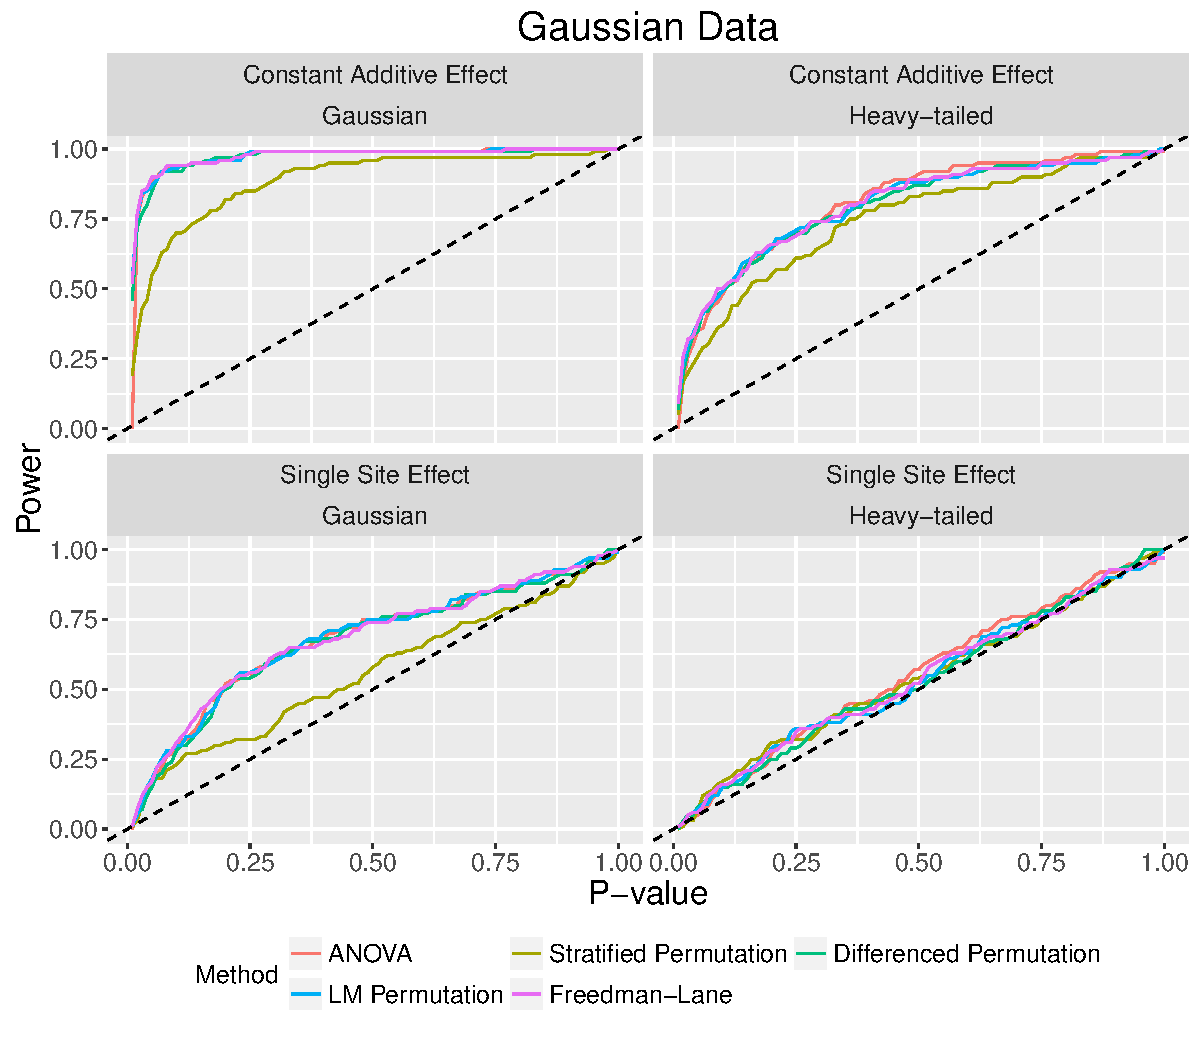
\includegraphics[width = \textwidth]{fig/normal_simulation_power}
\caption{Empirical power curves for the Gaussian simulated data}
\label{fig:normal_sim_power}
\end{figure}
\begin{center}
\begin{table}[ht]
\centering
\begin{tabular}{p{1.15in}|p{0.7in}|p{0.6in}p{0.8in}p{0.8in}p{0.8in}p{0.75in}}
  \hline
Treatment & Errors & ANOVA & Stratified Permutation & Differenced Permutation & LM Permutation & Freedman-Lane \\ 
  \hline
Constant Additive Effect & Gaussian & 0.89 & 0.55 & 0.86 & 0.89 & 0.89 \\ 
  Single Stratum Effect & Gaussian & 0.16 & 0.09 & 0.16 & 0.16 & 0.17 \\ 
  Constant Additive Effect & Heavy-tailed & 0.35 & 0.24 & 0.38 & 0.40 & 0.39 \\ 
  Single Stratum Effect & Heavy-tailed & 0.07 & 0.08 & 0.08 & 0.08 & 0.08 \\ 
   \hline
\end{tabular}
\caption{Empirical power at level $0.05$ for Gaussian simulated data} 
\label{tab:normal_power}
\end{table}

\end{center}

In our second set of simulations, we used the same design as the first simulations, but modified the sizes of the treatment groups.
Within each stratum, 4 individuals received one treatment and 12 received the second treatment.
This mimics real-world experiments, where the more expensive treatment is administered less frequently than the other.
It is well-known that both parametric and nonparametric tests have higher than nominal level when there is heterogeneous variance, and this effect is exaccerbated when group sizes are unequal (\cite{glass_consequences_1972}, \cite{zimmerman_two_2006}).
Here, the data have the same variance, so the test size should not be a problem, but power may suffer.\footnote{
See the supplementary simulation files for a treatment of heterogeneous variances.}
We omit a plot of the power curves from these simulations, as the patterns appear similar to those in Figure~\ref{fig:normal_sim_power}.
Table~\ref{tab:imbalanced_power} displays the value of these power curves and the size of the test at level $0.05$.
In this case, the permutation tests (except for the simple stratified permutation) have slightly higher power than the ANCOVA, but the difference is not substantial.
%\begin{figure}
%\centering
%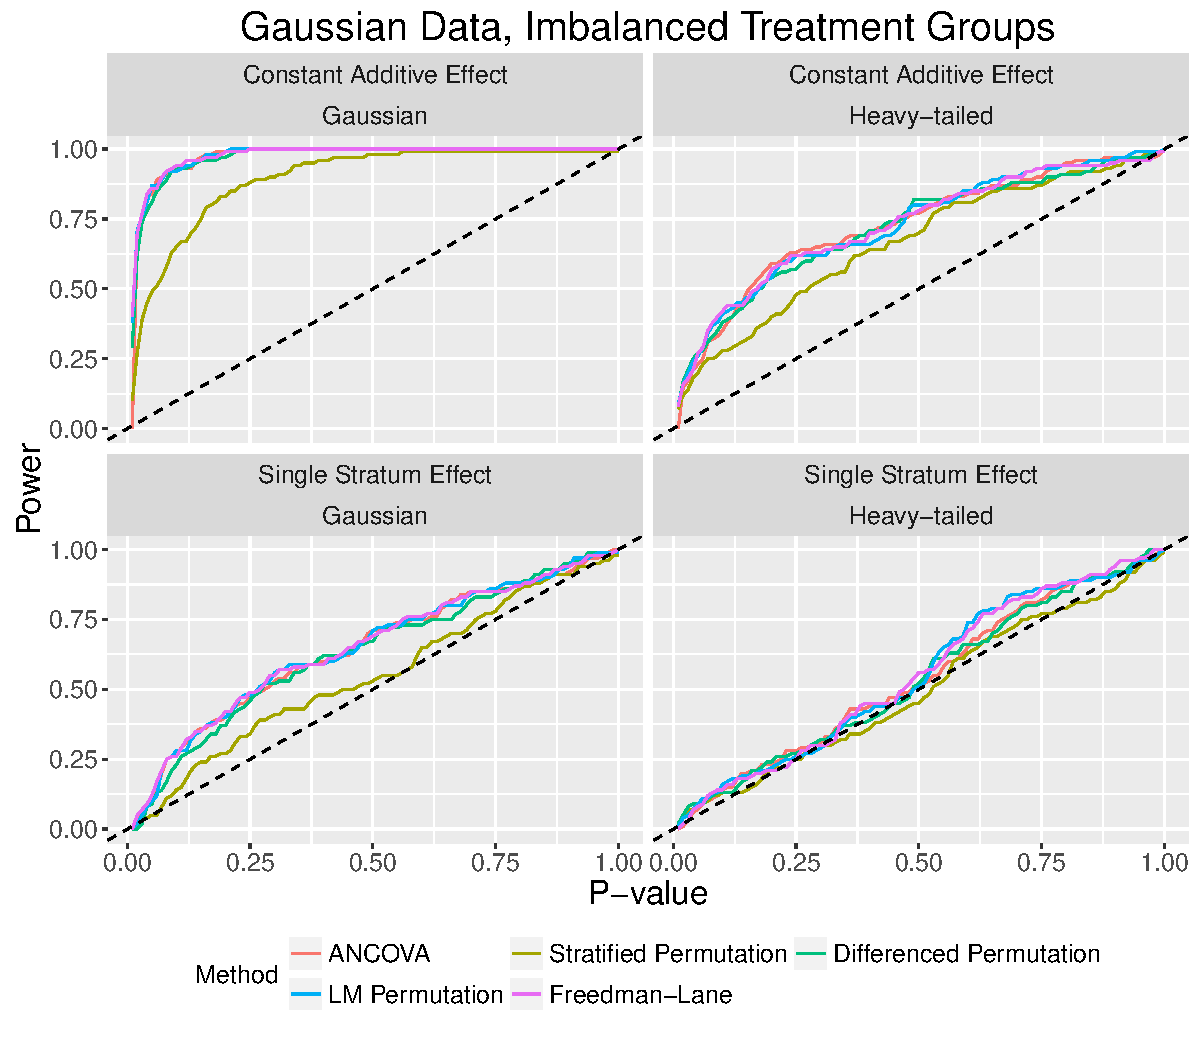
\includegraphics[width = \textwidth]{fig/imbalanced_simulation_power}
%\caption{Empirical power curves for the Gaussian simulated data with imbalanced group sizes}
%\label{fig:imbalanced_sim_power}
%\end{figure}
\begin{center}
\begin{table}[ht]
\centering
\begin{tabular}{|p{0.7in}|p{0.6in}p{0.8in}p{0.8in}p{0.8in}p{0.8in}p{0.75in}}
  \hline
Treatment & Errors & ANCOVA & Stratified Permutation & Differenced Permutation & LM Permutation & Freedman-Lane \\ 
  \hline
No Effect & Gaussian & 0.046 & 0.031 & 0.028 & 0.042 & 0.045 \\ 
  Constant Additive Effect & Gaussian & 0.840 & 0.490 & 0.810 & 0.870 & 0.860 \\ 
  Single Stratum Effect & Gaussian & 0.120 & 0.050 & 0.090 & 0.100 & 0.120 \\ 
   \hline
No Effect & Heavy-tailed & 0.034 & 0.054 & 0.055 & 0.047 & 0.042 \\ 
  Constant Additive Effect & Heavy-tailed & 0.230 & 0.200 & 0.270 & 0.260 & 0.270 \\ 
  Single Stratum Effect & Heavy-tailed & 0.070 & 0.080 & 0.090 & 0.090 & 0.080 \\ 
   \hline
\end{tabular}
\caption{Empirical power at level $0.05$ for Gaussian simulated data with imbalanced treatment groups} 
\label{tab:imbalanced_power}
\end{table}

\end{center}



In our third set of simulations, we assume that the baseline measurements $Y_{ij0}$ are discrete and skewed.
This is representative of some survey data, where individuals are asked to rate their experience on a scale from 1 to 10, for instance.
We generate the baseline measures using independent draws from a Poisson distribution with mean 4, and censoring values larger than 10, instead setting them to 10.
We condition on these observed baseline measures after we have generated them once.
Then, for each 1000 trials, we randomly assign treatment to half of the individuals in each stratum and generate errors taking on values $0.5$ and $-0.5$ with equal probability.
We construct $Y_{ij1}$ using Equation~\ref{eqn:dgp} with a treatment effect of $\gamma = 0.5$.
However we don't observe $Y_{ij1}$ but instead $\tilde{Y}_{ij1}$, which is defined as 

\begin{displaymath}
   \tilde{Y}_{ij1} = \left\{
     \begin{array}{ll}
       1 & \text{if } \tilde{Y}_{ij1} < 1\\
       10 & \text{if } \tilde{Y}_{ij1} > 10 \\
       \lfloor \tilde{Y}_{ij1} \rfloor & \text{otherwise}
     \end{array}
   \right.
\end{displaymath}

The observed outcomes $\tilde{Y}_{ij1}$, the baseline measures $Y_{ij0}$, and the errors are discrete.
The assumption of normality is clearly violated here.

We examine the effect of stratum size, rather than error distribution, in this set of simulations.
First, we consider balanced samples as before, where each stratum contains 16 individuals.
Next, we consider imbalanced strata, where the smallest stratum has only 8 individuals, the next has 16, and the largest has 24.
We again consider the four combinations of treatment effects and sample sizes.
In the case where there is only a non-null treatment effect in one stratum and sample sizes are different, this effect occurs in the smallest stratum.

Figure~\ref{fig:skewed_sim_power} shows the estimated power curves in these four designs.
When the treatment effect is constant, sample sizes within each stratum don't matter; the power curves look the same up to chance variation.
When the treatment effect only occurs in one stratum, there is a substantial loss in power because the effect only appears in the smallest stratum.
In practice, one does not usually know a priori which individuals will be affected by treatment (otherwise, those unaffected by treatment would be excluded from the study altogether),
This result suggests that when stratifying, one must be cautious not to stratify too finely, otherwise treatment effects may be indistinguishable from random variability.

As in the first set of simulations, the stratified permutation test using the raw outcomes has the lowest power of the five tests.
Now, however, the stratified permutation test using the difference between outcome and baseline also has lower power than the three using linear models.
Presumably, this is because the differences $\tilde{Y}_{ij1} - Y_{ij0}$ are also discrete and lie in a small range of values, so the test statistic does not vary greatly across permutations.
Table~\ref{tab:skewed_power} confirms this: power for the three linear model methods is high when the treatment is constant across strata, and power for all of the methods suffers when the effect is isolated in a single stratum.
All of the tests have lower than nominal level.


\begin{figure}
\centering
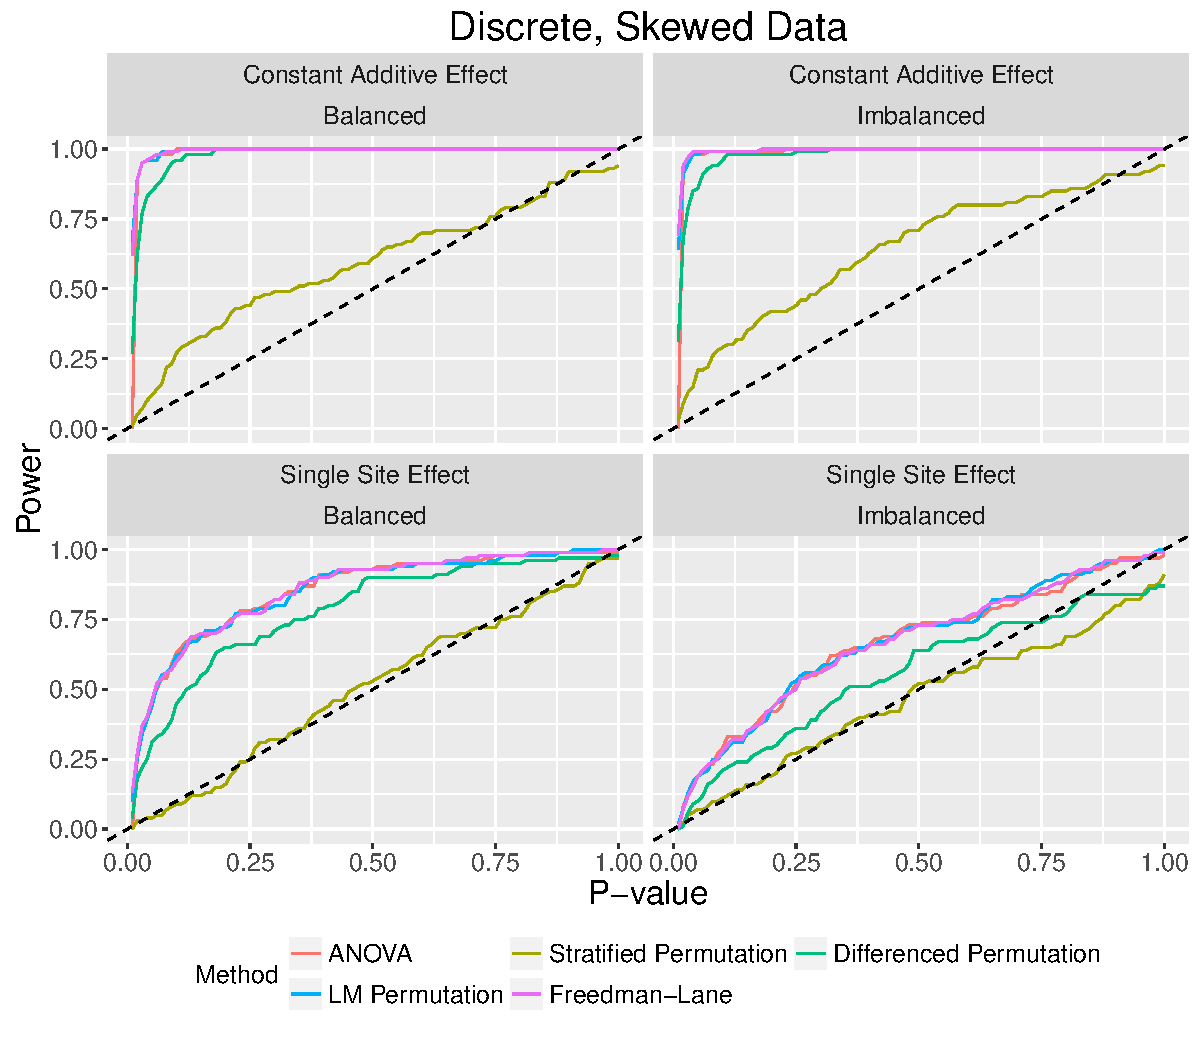
\includegraphics[width = \textwidth]{fig/skewed_simulation_power}
\caption{Empirical power curves for the skewed, discrete simulated data}
\label{fig:skewed_sim_power}
\end{figure}

\begin{center}
\begin{table}[ht]
\centering
\begin{tabular}{p{1.25in}|p{0.7in}|p{0.6in}p{0.8in}p{0.8in}p{0.8in}p{0.75in}}
  \hline
Treatment & Design & ANCOVA & Stratified Permutation & Differenced Permutation & LM Permutation & Freedman-Lane \\ 
  \hline
No Effect & Balanced & 0.036 & 0.025 & 0.021 & 0.035 & 0.037 \\ 
  Constant Additive Effect & Balanced & 0.974 & 0.143 & 0.853 & 0.972 & 0.977 \\ 
  Single Stratum Effect & Balanced & 0.422 & 0.050 & 0.275 & 0.429 & 0.424 \\ 
   \hline
No Effect & Imbalanced & 0.038 & 0.024 & 0.019 & 0.037 & 0.039 \\ 
  Constant Additive Effect & Imbalanced & 0.971 & 0.147 & 0.860 & 0.970 & 0.972 \\ 
  Single Stratum Effect & Imbalanced & 0.190 & 0.070 & 0.100 & 0.190 & 0.190 \\ 
   \hline
\end{tabular}
\caption{Empirical power at level $0.05$ for discrete, skewed simulated data} 
\label{tab:skewed_power}
\end{table}

\end{center}

It makes sense that in all of these simulations, the permutation test using the difference in outcome and baseline as the response measure is more powerful than the permutation test using the raw outcomes.
In additional simulations\footnote{see supplementary files on GitHub}, we modified the data-generating process given by Equation~\ref{eqn:dgp} so that the outcome and baseline had correlation of $0.25$.
In this case, the result was reversed: the differenced test had low power while the test using the raw outcomes had a power curve closer to the tests that adjust for covariates using a linear model.
This phenomenon has been studied before by \citet{frison_repeated_1992}, who recommended to use the difference in outcome and baseline if their correlation is greater than $0.5$ and to use the outcome only if their correlation is less than $0.5$.



\subsection{Clinical data results}
We compare the methods we discussed on a dataset from a clinical trial comparing the effectiveness of two treatments for gastroesophageal reflux disease (GERD).
Patients were treated at eight sites in two different countries.
At each site, patients were randomly assigned one of two treatments.
Patients were observed for a week before receiving treatment and for a week after receiving treatment.
On each of the fourteen days of observation, patients responded to a survey asking about their heartburn, regurgitation, and dyspepsia frequency and severity.
These endpoints are measured on a discrete scale.
There were several additional derived endpoints, such as daily regurgitation, daily ``hrdq'', and daily dyspepsia, which are functions of the survey measures.
Daily ``hrdq'' was the primary endpoint.
To reduce day-to-day variation, we averaged the measures in the pretreatment week and post-treatment week for each endpoint.

In our model, we treat site as the stratification variable, as this is the level at which treatment was randomized.
We do not include country in the model, as a country-level effect should be captured in the site-level effects.
The linear model for ANCOVA analysis is as in Equation~\ref{eqn:ancova}.
We chose to use this form of the model, with the actual outcomes as the $Y$ and the baseline measures as control variables, rather than testing the difference in outcome and baseline. 
The outcome and baseline had a low correlation (for instance, $0.56$ for daily ``hrdq''), so we did not use their difference as the dependent variable. 
As our simulations and previous work (\cite{frison_repeated_1992}) show, when the correlation between baseline and outcome is low, it is more powerful to control for baseline outcomes using a model.

Figure~\ref{fig:clinical_distr} shows the distribution of each clinical endpoint, separated by treatment group.
There is a clear visual difference in distributions for daily heartburn (``daily\_heart''), daily ``hrdq'', and heartburn frequency (``heart\_freq'').
The difference is less clear for daily regurgitation (``daily\_regurg'') and regurgitation frequency (``regurg\_freq'').

Table~\ref{tab:clinical_pvalues} shows the $p$-values for the four tests.
Overall, the results confirm our expectations based on visual comparison in Figure~\ref{fig:clinical_distr}:
one or more of the tests reject the null hypothesis that outcomes are the same between treatments for heartburn frequency, daily heartburn, and daily ``hrdq,''
but not for any of the other endpoints.
The three tests based on the linear model all give similar results here.
The $p$-values for the ANCOVA tend to be smaller than the linear model and the residual permutation tests, while the $p$-values stratified, unadjusted permutation test have no consistent pattern.
These results match our simulations: the parametric test has comparable or slightly higher power than the other permutation tests.

\begin{figure}
\centering
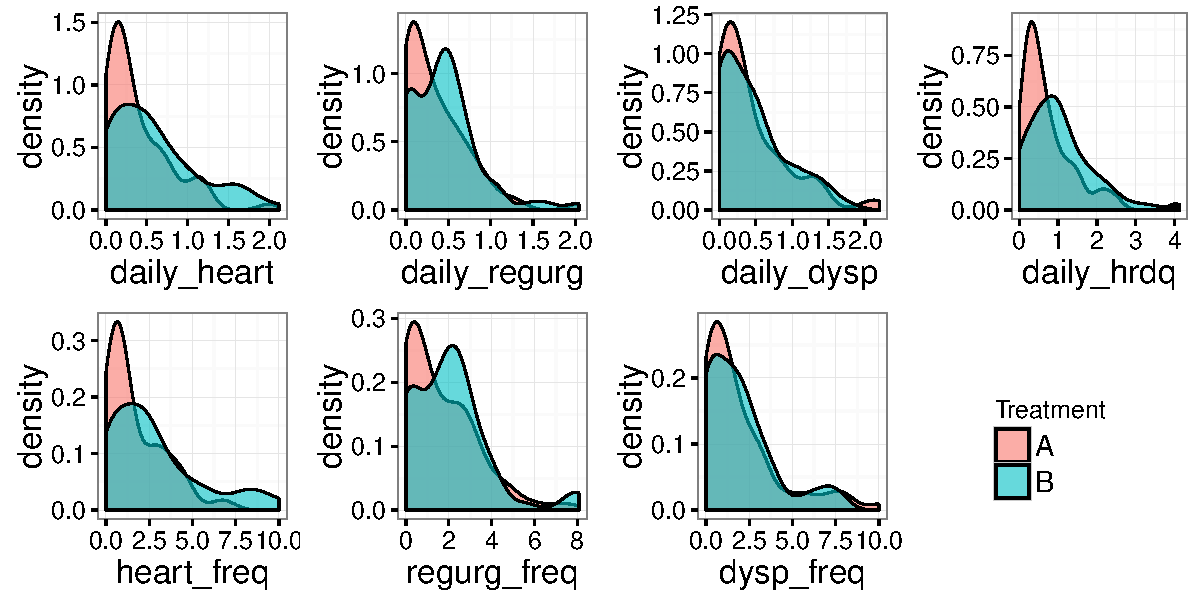
\includegraphics[width = \textwidth]{fig/clinical_distr}
\caption{Distribution of each endpoint for the two treatments A and B}
\label{fig:clinical_distr}
\end{figure}


\begin{center}
\begin{table}[ht]
\centering
\begin{tabular}{r|p{1.2in}p{1.2in}p{1.2in}p{1.2in}}
  \hline
 & Parametric ANCOVA & Stratified permutation & LM permutation & Residual permutation \\ 
  \hline
heart\_freq & 0.035 & 0.006 & 0.080 & 0.082 \\ 
  regurg\_freq & 0.136 & 0.118 & 0.280 & 0.220 \\ 
  dysp\_freq & 0.565 & 0.948 & 0.616 & 0.592 \\ 
  daily\_heart & 0.032 & 0.004 & 0.056 & 0.068 \\ 
  daily\_regurg & 0.142 & 0.174 & 0.286 & 0.246 \\ 
  daily\_hrdq & 0.043 & 0.012 & 0.088 & 0.098 \\ 
  daily\_dysp & 0.582 & 0.810 & 0.756 & 0.722 \\ 
   \hline
\end{tabular}
\caption{Comparison of p-values from four tests, for each continuous endpoint.} 
\label{tab:clinical_pvalues}
\end{table}

\end{center}

\section{Discussion}
% This section should discuss the implications of the findings in context of existing research and highlight limitations of the study.

\bit
\item This paper adds to the literature comparing parametric and nonparametric tests.
Our results match those of \citet{vickers_parametric_2005}, where he found that ANCOVA performed the same or better than nonparametric tests.
\item Results about differenced vs raw outcomes. This isn't new but our simulations and empirical dataset confirm it in the context of permutation tests
\item In an ideal case, one knows all covariates related to the outcome and fits a fully saturated linear model (including all covariates and their interactions), the coefficient for the treatment is an asymptotically consistent estimate of the average treatment effect (\cite{lin_agnostic_2013}).
\item Permutation tests don't come free of assumptions, though.  \citet{romano_behavior_1990} warns against using permutation tests naively, if items are not truly exchangeable. For instance, he points to the case where observations have unequal variances.  \citet{boik_fisherpitman_1987} illustrates this phenomenon, comparing the normal theory $F$ test to its permutation counterpart and demonstrating by simulation that the latter has larger than nominal level.
\item Errors are very important!  They are a source of non-exchangeability.  We can't observe them, so we need to believe that they are actually homogeneous and do some checks on residuals to give evidence.
\bit
\item \citet{gail_tests_1988} propose a randomization test based on residuals, using not a linear model but an exponential family model to construct residuals, and find that omitting relevant covariates leads to tests with higher than nominal level.  \todo{perhaps this is something that one should be mindful of when using these linear model based tests.}
\item Freedman-Lane stuff: for the appro
In randomized experiements, we are guaranteed that treatment $Z$ is independent of $\varepsilon$, conditional on stratum.
Indeed, the distribution of residuals looks nearly equal between treatment groups in both models.
As mentioned, this should not be an issue since we permute treatments within sites, independently across sites.
(In general, when treatment is not randomly assigned, this condition is necessary for the permutation test to be valid.)
\eit
\eit


% list of abbreviations

\section{Declarations}
% see http://bmcmedresmethodol.biomedcentral.com/submission-guidelines/preparing-your-manuscript/technical-advance-article
\textbf{Ethics approval and consent to participate}
Not applicable
\textbf{Consent for publication}
\textbf{Availability of data and material}
\textbf{Competing interests}
\textbf{Funding}
\textbf{Authors' contributions}
\textbf{Acknowledgements}
\textbf{Authors' information}

\bibliographystyle{plainnat}
\bibliography{references}




\end{document}